%
%===============>>  ГРУППА 5-1 МОДУЛЬ 2  <<=============
%
\setmodule{2} 

%BEGIN_FOLD % ====>>_____ Занятие 1 _____<<====
\begin{class}[number=1]
\begin{listofex}
	\item Какие числа называют простыми? Какие составными?
	\item Выберите из данных числе простые:
	\begin{tasks}(10)
		\task \( 4 \)
		\task \( 15 \)
		\task \( 7 \)
		\task \( 17 \)
		\task \( 27 \)
		\task \( 51 \)
		\task \( 37 \)
		\task \( 81 \)
		\task \( 57 \)
		\task \( 67 \)
	\end{tasks}
	\item Представьте составное число в виде произведения простых:
	\begin{tasks}(3)
		\task \( 24 \)
		\task \( 36 \)
		\task \( 30 \)
		\task \( 50 \)
		\task \( 98 \)
		\task \( 288 \)
		\task \( 1000 \)
		\task \( 520 \)
		\task \( 225 \)
	\end{tasks}
	\item Найдите наибольший общий делитель двух чисел:
	\begin{tasks}(4)
		\task НОД\( (30;\;25) \)
		\task НОД\( (24;\;40) \)
		\task НОД\( (60;\;88) \)
		\task НОД\( (81;\;108) \)
		\task НОД\( (24;\;40) \)
		\task НОД\( (20;\;100) \)
		\task НОД\( (23;\;61) \)
		\task НОД\( (4;\;92) \)
	\end{tasks}
	\item Найдите наибольший общий делитель трех чисел:
	\begin{tasks}(2)
		\task НОД\( (66;\;44;\;88) \)
		\task НОД\( (64;\;80;\;44) \)
	\end{tasks}
	\item Найдите наименьшее общее кратное двух чисел:
	\begin{tasks}(2)
		\task НОК\( (30;\;25) \)
		\task НОК\( (24;\;40) \)
		\task НОК\( (60;\;88) \)
		\task НОК\( (20;\;100) \)
	\end{tasks}
	\end{listofex}
\end{class}
%END_FOLD

%BEGIN_FOLD % ====>>_____ Занятие 2 _____<<====
\begin{class}[number=2]
	\begin{listofex}
	\item Разделите простые и составные числа на две группы:
	\[ 12,\;13,\;25,\;31,\;261,\;19,\;7,\;61,\;121,\;2,\;39,\;61,\;150 \]
	\item Расположите числа в порядке возрастания:
	\[ 50057,\;507,\;5757,\;77755,\;75057,\;7557,\;55577,\;7057,\;570 \]
	\item Вместо звёздочки подставьте, если возможно, цифру так, чтобы получилось правильное
	неравенство:
	\begin{tasks}(3)
		\task \( 3128 < 312\:* \)
		\task \( 5782 > 57*2 \)
		\task \( 38*46 < 38300 \)
	\end{tasks}
	\item Разложите на простые множители:
	\begin{tasks}(4)
		\task \( 84 \)
		\task \( 112 \)
		\task \( 280 \)
		\task \( 4500 \)
	\end{tasks}
	\item Найдите:
	\begin{tasks}(2)
		\task НОД\( (45;\;60) \)
		\task НОД\( (27;\;36) \)
		\task НОД\( (54;\;36) \)
		\task НОД\( (220;\;180) \)
	\end{tasks}
	\item Найдите:
	\begin{tasks}(2)
		\task НОК\( (45;\;60) \)
		\task НОК\( (27;\;36) \)
		\task НОК\( (34;\;51) \)
		\task НОК\( (120;\;150) \)
	\end{tasks}
	\item Шоколадка стоит \( 35 \) рублей. В воскресенье в супермаркете действует специальное
	предложение: заплатив за две шоколадки, покупатель получает три (одну в подарок). Сколько
	шоколадок можно получить на \( 200 \) рублей в воскресенье?
	\end{listofex}
\end{class}
%END_FOLD

%BEGIN_FOLD % ====>>_ Домашняя работа 1 _<<====
\begin{homework}[number=1]
	\begin{listofex}
	\item Найдите:
	\begin{tasks}(2)
		\task НОД\( (48;\;72) \)
		\task НОД\( (36;\;42) \)
		\task НОК\( (48;\;72) \)
		\task НОК\( (36;\;42) \)
	\end{tasks}
	\item Ответе на вопросы:
	\begin{tasks}
		\task Сколько часов в одной шестой суток?
		\task Сколько метров в одной четверти километра?
		\task Сколько минут в половине часа?
		\task Сколько грамм в \( \dfrac{1}{10} \) килограмма?
		\task Сколько метров в \( \dfrac{3}{5} \) километра?
	\end{tasks}
	\item Постройте в тетради отрезок \( AB \) длинной \( 16 \) см. Отметьте на этом отрезке точки \( C,\;D,\;E \) так, чтобы \( AC=\dfrac{1}{4}AB;\;AD=\dfrac{3}{8}AB;\;AE=\dfrac{13}{16}AB \)
	\item Потратили \( \dfrac{7}{9} \) от \( 350 \) руб. Сколько рублей осталось?
	\item У брата и сестры вместе \( 28 \) открыток. Сестра отдала брату \( 4 \) открытки, и открыток у них стало поровну. Сколько открыток было у каждого из них сначала?
	\item Для компота купили \( 1800 \) г. сухофруктов. Яблоки составляют \( 4 \) части, груши --- 3 части, а сливы --- 2 части от общего веса сухофруктов. Сколько граммов яблок, груш и слив было в отдельности?
	\item Вычислить:
	\begin{tasks}(4)
		\task \( \dfrac{1}{5} \) от \( 100 \)
		\task \( \dfrac{3}{7} \) от \( 84 \)
		\task \( \dfrac{11}{8} \) от \( 88 \)
		\task \( \dfrac{14}{25} \) от \( 225 \)
	\end{tasks}
	\end{listofex}
\end{homework}
%END_FOLD

%BEGIN_FOLD % ====>>_____ Занятие 3 _____<<====
\begin{class}[number=3]
	\begin{listofex}
	\item Что такое обыкновенная дробь?
	\item Ответьте на вопросы:
	\begin{tasks}
		\task Сколько часов в одной трети суток?
		\task Сколько метров в одной восьмой километра?
		\task Сколько минут в четверти часа?
		\task Сколько миллиметров в \( \dfrac{1}{2} \) сантиметра?
		\task Сколько минут в \( \dfrac{2}{3} \) часа?
	\end{tasks}
	\item Постройте в тетради отрезок \( AB \) длинной \( 12 \) см. Отметьте на этом отрезке точки \( C,\;D,\;E \) так, чтобы \( AC=\dfrac{1}{3}AB;\;AD=\dfrac{1}{4}AB;\;AE=\dfrac{5}{6}AB \)
	\item Постройте квадрат со стороной 6 клеток. Закрасьте \( \dfrac{2}{3} \) часть квадрата.
\end{listofex}
\begin{definit}
	\textbf Чтобы найти часть \( \frac{a}{b} \) от числа \( c \), необходимо число \( c \) поделить на \( b \) и потом полученный результат умножить на \( a \).
\end{definit}
\begin{listofex}[start=5]
	\item Потратили \( \dfrac{3}{8} \) от \( 400 \) руб. Сколько рублей потратили?
	\item Длина веревки \( 27 \) м. Отрезали \( \dfrac{2}{9} \) ее длины. Сколько метров веревки отрезали? Сколько осталось?
	\item Вычислить:
	\begin{tasks}(4)
		\task \( \dfrac{1}{4} \) от \( 64 \)
		\task \( \dfrac{3}{5} \) от \( 25 \)
		\task \( \dfrac{17}{11} \) от \( 121 \)
		\task \( \dfrac{5}{6} \) от \( 196 \)
	\end{tasks}
	\item Туристам необходимо пройти \( 24 \) км за три дня. В первый день они прошли \( \dfrac{9}{24} \) от запланированного пути, а во второй день \( \dfrac{1}{4} \) от всего пути. Сколько им осталось пройти в третий день?
	\item Ученик решил сделать домашнюю работу по математике за два дня. В первый день он сделал \( \dfrac{7}{18} \) от всей работы, а во второй день \( \dfrac{4}{6} \) от всей работы. Возможно ли такое?
	\item Работу выполнили за 4 ч. Какую часть работы выполняли за каждый час, если работали равномерно и без перерывов?
	\item За каждый час труба наполняет \( \dfrac{2}{6} \) бассейна. За сколько часов она наполнит весь бассейн?
	\end{listofex}
\end{class}
%END_FOLD

%BEGIN_FOLD % ====>>_____ Занятие 4 _____<<====
\begin{class}[number=4]
	\begin{listofex}
	\item Ответе на вопросы:
	\begin{tasks}
		\task Сколько часов в одной четверти суток?
		\task Сколько метров в одной десятой километра?
		\task Сколько минут в третей часа?
		\task Сколько миллиметров в \( \dfrac{1}{5} \) сантиметра?
		\task Сколько часов в \( \dfrac{5}{6} \) часа?
	\end{tasks}
	\item Постройте в тетради отрезок \( AB \) длинной \( 20 \) см. Отметьте на этом отрезке точки \( C,\;D,\;E \) так, чтобы \( AC=\dfrac{1}{4}AB;\;AD=\dfrac{3}{5}AB;\;AE=\dfrac{7}{10}AB \)
	\item Постройте прямоугольник со сторонами \( 6 \) и \( 8 \) клеток. Закрасьте \( \dfrac{3}{8} \) часть квадрата.
	\item Потратили \( \dfrac{12}{30} \) от \( 300 \) руб. Сколько рублей потратили?
	\item Длина поезда \( 500 \) м., а длина одного вагона \( 50 \) м. Отцепили \( \dfrac{4}{10} \) всех вагонов. Какая стала длина состава? Сколько вагонов осталось?
	\item Вычислить:
	\begin{tasks}(4)
		\task \( \dfrac{1}{4} \) от \( 80 \)
		\task \( \dfrac{2}{7} \) от \( 35 \)
		\task \( \dfrac{51}{15} \) от \( 75 \)
		\task \( \dfrac{11}{12} \) от \( 288ы \)
	\end{tasks}
	\item Туристам необходимо пройти \( 48 \) км за три дня. В первый день они прошли \( \dfrac{5}{12} \) от запланированного пути, а во второй день \( \dfrac{1}{4} \) от всего пути. Сколько им осталось пройти в третий день?
	\item за первую неделю месяца, менеджер выполнил \( \dfrac{3}{7} \) плана продаж, а за вторую неделю \( \dfrac{1}{5} \), какую часть плана ему осталось выполнить за вторые две недели месяца?
	\item Работу выполнили за 12 ч. Какую часть работы выполняли за каждый час, если работали равномерно и без перерывов? Какую часть работы выполнят через 4 часа от начала работы?
	\item За каждый час труба наполняет \( \dfrac{4}{20} \) бассейна. За сколько часов она наполнит весь бассейн?
	\end{listofex}
\end{class}
%END_FOLD

%BEGIN_FOLD % ====>>_____ Занятие 5 _____<<====
\begin{class}[number=5]
	\begin{listofex}
	\item \textbf{Основное свойство дроби}
	
	Если числитель и знаменатель дроби увеличить или уменьшить в одно и тоже количество раз, то значение дроби не изменится.
	\item Сократить дробь:
	\begin{tasks}(2)
		\task \( \dfrac{12}{16} \)
		\task \( \dfrac{15}{25} \)
	\end{tasks}
	\item Привести к общему знаменателю:
	\begin{tasks}(4)
		\task \( \dfrac{4}{25} \) и \( \dfrac{1}{5} \)
		\task \( \dfrac{3}{17} \) и \( \dfrac{2}{34} \)
		\task \( \dfrac{10}{9} \) и \( \dfrac{5}{3} \)
		\task \( \dfrac{3}{24} \) и \( \dfrac{1}{12} \)
		\task \( \dfrac{5}{20} \) и \( \dfrac{13}{50} \)
		\task \( \dfrac{6}{25} \) и \( \dfrac{13}{75} \)
		\task \( \dfrac{15}{24} \) и \( \dfrac{16}{36} \)
		\task \( \dfrac{1}{33} \) и \( \dfrac{1}{55} \)
		\task \( \dfrac{4}{11} \) и \( \dfrac{16}{121} \)
		\task \( \dfrac{24}{100} \) и \( \dfrac{13}{4} \)
		\task \( \dfrac{11}{90} \) и \( \dfrac{33}{50} \)
		\task \( \dfrac{13}{250} \) и \( \dfrac{14}{350} \)
	\end{tasks}
	\item Сравнить дроби:
	\begin{tasks}(4)
		\task \( \dfrac{5}{7} \) и \( \dfrac{2}{3} \)
		\task \( \dfrac{5}{12} \) и \( \dfrac{7}{16} \)
		\task \( \dfrac{33}{15} \) и \( \dfrac{23}{12} \)
		\task \( \dfrac{13}{21} \) и \( \dfrac{15}{28} \)
		\task \( \dfrac{131}{200} \) и \( \dfrac{54}{100} \)
		\task \( \dfrac{37}{50} \) и \( \dfrac{97}{150} \)
		\task \( \dfrac{33}{13} \) и \( \dfrac{45}{15} \)
		\task \( \dfrac{15}{70} \) и \( \dfrac{1}{30} \)
	\end{tasks}
	\end{listofex}
\end{class}
%END_FOLD

%BEGIN_FOLD % ====>>_____ Занятие 6 _____<<====
\begin{class}[number=6]
	\begin{listofex}
	\item Сократить дробь:
	\begin{tasks}(6)
		\task \( \dfrac{12}{16} \)
		\task \( \dfrac{10}{14} \)
		\task \( \dfrac{15}{25} \)
		\task \( \dfrac{32}{48} \)
		\task \( \dfrac{32}{128} \)
		\task \( \dfrac{18}{27} \)
		\task \( \dfrac{17}{170} \)
		\task \( \dfrac{20}{36} \)
		\task \( \dfrac{15}{35} \)
		\task \( \dfrac{36}{92} \)
		\task \( \dfrac{42}{66} \)
		\task \( \dfrac{27}{63} \)
	\end{tasks}
	\item Сократить дробь:
	\begin{tasks}(6)
		\task \( \dfrac{75}{90} \)
		\task \( \dfrac{168}{216} \)
		\task \( \dfrac{60}{144} \)
		\task \( \dfrac{255}{285} \)
		\task \( \dfrac{148}{185} \)
		\task \( \dfrac{143}{121} \)
	\end{tasks}
	\item Привести:
	\begin{tasks}(2)
		\task \( \dfrac{3}{4} \) к знаменателю \( 20 \)
		\task \( \dfrac{5}{7} \) к знаменателю \( 63 \)
		\task \( \dfrac{11}{12} \) к знаменателю \( 144 \)
		\task \( \dfrac{9}{20} \) к знаменателю \( 160 \)
		\task \( \dfrac{11}{9} \) к знаменателю \( 99		 \)
		\task \( \dfrac{4}{15} \) к знаменателю \( 60 \)
		\task \( \dfrac{13}{14} \) к знаменателю \( 56 \)
	\end{tasks}
	\item Сравнить дроби:
	\begin{tasks}(4)
		\task \( \dfrac{5}{7} \) и \( \dfrac{2}{3} \)
		\task \( \dfrac{5}{12} \) и \( \dfrac{7}{16} \)
		\task \( \dfrac{33}{15} \) и \( \dfrac{23}{12} \)
		\task \( \dfrac{13}{21} \) и \( \dfrac{15}{28} \)
		\task \( \dfrac{131}{200} \) и \( \dfrac{54}{100} \)
		\task \( \dfrac{37}{50} \) и \( \dfrac{97}{150} \)
		\task \( \dfrac{33}{13} \) и \( \dfrac{45}{15} \)
		\task \( \dfrac{15}{70} \) и \( \dfrac{1}{30} \)
	\end{tasks}
	\item Сократить дробь:
	\begin{tasks}(5)
		\task \( \dfrac{7\cdot3}{3\cdot14} \)
		\task \( \dfrac{14\cdot9}{6\cdot7\cdot3} \)
		\task \( \dfrac{25\cdot99}{81\cdot55} \)
		\task \( \dfrac{16\cdot45\cdot19}{81\cdot57\cdot4} \)
		\task \( \dfrac{3\cdot14\cdot62}{31\cdot10\cdot27} \)
	\end{tasks}
	\end{listofex}
\end{class}
%END_FOLD

%BEGIN_FOLD % ====>>_____ Занятие 7 _____<<====
\begin{class}[number=7]
	\title{Подготовка к проверочной}
	\begin{listofex}
	\item Чем отличаются простые числа от составных?
	\item Разложите на простые множители:
	\begin{tasks}(2)
		\task \( 96 \)
		\task \( 132 \)
	\end{tasks}
	\item Найдите:
	\begin{tasks}(2)
		\task НОД\( (36;\;60) \)
		\task НОК\( (54;\;72) \)
	\end{tasks}
	\item Вместо звёздочки подставьте, если возможно, цифру так, чтобы получилось правильное
	неравенство:
	\begin{tasks}(3)
		\task \( 4328 < 432\:* \)
		\task \( 34182 > 34*52 \)
		\task \( 18*00 < 18100 \)
	\end{tasks}
	\item Сколько сантиметров в четверти метра? Какую часть составляет 3 часа от дня?
	\item Вычислить:
	\begin{tasks}(4)
		\task \( \dfrac{1}{4} \) от \( 16 \)
		\task \( \dfrac{3}{5} \) от \( 75 \)
		\task \( \dfrac{13}{50} \) от \( 10000 \)
		\task \( \dfrac{25}{36} \) от \( 288 \)
	\end{tasks}
	\item Потратили \( \dfrac{3}{15} \) от \( 7500 \) руб. Сколько рублей потратили? Сколько рублей осталось?
	\item Рабочим поручено отремонтировать участок дороги за три дня. В первый день они отремонтировали \( \dfrac{4}{15} \) от всего участка дороги, а во второй день -- \( \dfrac{7}{15} \) от всего участка. Какую часть дороги им осталось отремонтировать в третий день?
	\item Каждый час труба наполняет \( \dfrac{4}{20} \) бассейна. За сколько часов труба наполин весь бассейн?
	\item Сформулируйте основное свойство дроби.
	\item Сократить дробь:
	\begin{tasks}(5)
		\task \( \dfrac{15}{30} \)
		\task \( \dfrac{22}{77} \)
		\task \( \dfrac{26}{39} \)
		\task \( \dfrac{132}{286} \)
		\task \( \dfrac{520}{1040} \)
	\end{tasks}
	\item Привести:
	\begin{tasks}(4)
		\item \( \dfrac{2}{5} \) к знам-лю \( 40 \)
		\item \( \dfrac{1}{12} \) к знам-лю \( 72 \)
		\item \( \dfrac{14}{7} \) к знам-лю \( 63 \)
		\item \( \dfrac{4}{18} \) к знам-лю \( 234 \)
	\end{tasks}
	\item Сократить дробь:
	\begin{tasks}(4)
		\task \( \dfrac{5\cdot12}{3\cdot25} \)
		\task \( \dfrac{33\cdot8}{22\cdot2\cdot3} \)
		\task \( \dfrac{225\cdot34}{30\cdot17} \)
		\task \( \dfrac{32\cdot64\cdot16}{16\cdot4\cdot8} \)
	\end{tasks}
	\end{listofex}
\end{class}
%END_FOLD

%BEGIN_FOLD % ====>>_ Проверочная работа _<<====
\begin{exam}
	\begin{listofex}
	\item Разложите на простые множители:
	\begin{tasks}(2)
		\task \( 75 \)
		\task \( 260 \)
	\end{tasks}
	\item Найдите:
	\begin{tasks}(2)
		\task НОД\( (24;\;30) \)
		\task НОК\( (39;\;78) \)
	\end{tasks}
	\item Вместо звёздочки подставьте, если возможно, цифру так, чтобы получилось правильное
	неравенство:
	\begin{tasks}(2)
		\task \( 12798 < 12*98 \)
		\task \( 21415 > 2*415 \)
	\end{tasks}
	\item Сколько минут в трети часа? Какую часть составляют 20 см от метра?
	\item Вычислить:
	\begin{tasks}(4)
		\task \( \dfrac{1}{8} \) от \( 56 \)
		\task \( \dfrac{4}{9} \) от \( 99 \)
		\task \( \dfrac{29}{50} \) от \( 100 \)
		\task \( \dfrac{16}{14} \) от \( 126 \)
	\end{tasks}
	\item Потратили \( \dfrac{4}{25} \) от \( 5000 \) руб. Сколько рублей потратили? Сколько рублей осталось?
	\item Товарный поезд за три дня должен перевезти груз из пункта \( A \) в пункт \( B \). В первый день он проехал \( \dfrac{6}{17} \) от всего пути, а во второй --- \( \dfrac{7}{17} \) от всего пути. Какую часть пути ему осталось проехать в третий день?
	\item Каждый час Антон красит \( \dfrac{3}{18} \) забора. За сколько часов Антон покрасит весь забор?
	\item Сократить дробь:
	\begin{tasks}(5)
		\task \( \dfrac{14}{20} \)
		\task \( \dfrac{24}{64} \)
		\task \( \dfrac{33}{121} \)
		\task \( \dfrac{50}{750} \)
		\task \( \dfrac{3500}{20000} \)
	\end{tasks}
	\item Привести:
	\begin{tasks}(3)
		\task \( \dfrac{2}{7} \) к знам-лю \( 49 \)
		\task \( \dfrac{1}{13} \) к знам-лю \( 78 \)
		\task \( \dfrac{57}{40} \) к знам-лю \( 120 \)
	\end{tasks}
	\item Сократить дробь:
	\begin{tasks}(4)
		\task \( \dfrac{6\cdot7}{3\cdot7} \)
		\task \( \dfrac{12\cdot16}{32\cdot4} \)
		\task \( \dfrac{55\cdot16}{11\cdot10\cdot8} \)
		\task \( \dfrac{144\cdot60}{20\cdot72} \)
	\end{tasks}
	\end{listofex}
\end{exam}
%END_FOLD

%BEGIN_FOLD % ====>>_ Консультация _<<====
\begin{consultation}
\begin{listofex}
	\item Сумма пяти различных натуральных (то есть целых положительных) чисел равна 100. Какое
	наибольшее значение может принимать самое больше из этих чисел?
	\item Прямоугольник на рисунке составлен из 7 квадратов. Сторона каждого закрашенного квадрата
	равна 4см. Чему равна сторона большого белого квадрата?
	\begin{center}
		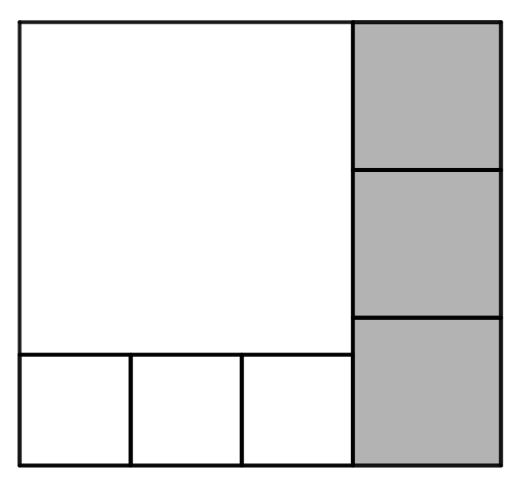
\includegraphics[align=t, width=\linewidth]{\picpath/124}
	\end{center}
	\item Незнайка хотел купить пять порций мороженого, но ему не хватило 80 рублей. Тогда он купил две порции мороженого, и у него осталось 70 рублей. Сколько денег было у Незнайки изначально?
	\item На доске выписаны в порядке возрастания все пятизначные числа, в записи которых используются
	пять последовательных цифр. Какое число идет после \( 59876 \)?
	\item Малыш, Карлсон и Винни-Пух съели торт. Они ели одновременно и каждый ел торт с одной и
	той же скоростью. Малышу досталась только \( 1/13 \) часть торта. А вот если бы Малыш ел только с Карлсоном, то ему бы досталась четверть торта. Какую долю торта съел бы Малыш, если бы он ел только с Винни-Пухом? (В ответе укажите такое число \( N \), что Малышу достанется \( 1/N \) часть торта)

	\item Решить ребус: ЦВЕТОК \( + \) ЦВЕТОК \( + \) ЦВЕТОК \( = \) БУКЕТИК
\end{listofex}
\end{consultation}
%END_FOLD

%BEGIN_FOLD % ====>>_ Консультация _<<====
\begin{consultation}
	\begin{listofex}
	\item Средний день первой половины сентября --- среда. Каким днем недели будет средний день второй половины сентября?
	\item В числе \( 437 \) попугай Кеша поменял местами две цифры, а потом одну цифру стер. Какой наибольшее двухзначное число могло получиться?
	\item Из двух диаметрально противоположных точек кругового трека стартовали в одном направлении два велосипедиста. Они едут с постоянными скоростями, при этом скорость у одного из велосипедистов больше, поэтому время от времени он обгоняет второго. Шестой обгон случился через \( 33 \) минуты после старта. Через сколько минут после шестого обгона случится седьмой обгон?
	\item Сумма пяти различных натуральных чисел равна \( 300 \). Какое наибольшее значение может принимать самое большое из этих чисел?
	\item На некоторых деревьях в волшебном лесу растут монеты. Деревьев, на которых вообще не растут монеты, в два раза больше, чем деревьев, на которых растут по
	три монеты. На трёх деревьях растут по \( 2 \) монеты, на четырёх деревьях — по \( 4 \) монеты, а
	больше, чем по \( 4 \) монеты, ни на каком дереве не растёт. На сколько общее число монет в
	волшебном лесу больше, чем число деревьев?
\end{listofex}
\end{consultation}
%END_FOLD

%BEGIN_FOLD % ====>>_ Консультация _<<====
\begin{consultation}
	\begin{listofex}
	\item Из города \( N \) одновременно в одном направлении выехали два автомобиля. Скорость
	одного из них равна \( 101 \) км/ч. Через \( 4 \) часа после начала движения расстояние между
	автомобилями оказалось равно \( 108 \) км. Найдите скорость второго автомобиля. Подумайте,
	сколько решений имеет задача.
	\item Города \( A \) и \( B \) расположены на одном шоссе на расстоянии \( 70 \) км. Из города \( A \) в направлении города \( B \) выезжает автомобиль со скоростью \( 80 \) км/ч. Одновременно из города \( B \) в том же направлении выезжает другой автомобиль. Найдите скорость второго автомобиля, если через \( 3 \) часа после начала движения расстояние между автомобилями оказалось равно \( 10 \) км.
	\item Из поселка вышел пешеход со скоростью \( 6 \) км/ч, а через \( 4 \) часа вслед за ним выехал велосипедист, скорость которого \( 18 \) км/ч. Через сколько часов после выхода пешехода его догонит велосипедист? На каком расстоянии от поселка произойдет встреча?
	\item Расстояние между пунктами \( A \) и \( B \) , расположенными на одной реке, равно \( 60 \) км. Из пунктов \( A \) и \( B \) одновременно навстречу друг другу выплывают две моторные лодки. Собственная скорость каждой лодки равна \( 15 \) км/ч. Скорость течения реки равна \( 2 \) км/ч. Через какое время после начала движения и на каком расстоянии от каждого из пунктов лодки встретятся?
	\item От пристани \( A \) против течения реки выплывает пароход, собственная скорость которого равна \( 20 \) км/ч. Скорость течения реки равна \( 4 \) км/ч. Через \( 2 \) часа
	после начала движения пароход сломался и его течением стало сносить обратно к пристани \( A \).
	Через сколько часов после начала движения пароход снова окажется у пристани \( A \)?
	\item Из пункта \( A \) круговой трассы, длина которой \( 96 \) км, одновременно в одном направлении стартовали два автогонщика. Скорость первого гонщика \( 182 \) км/ч, а скорость
	второго --- \( 166 \) км/ч. Через какое время первый гонщик будет опережать второго ровно на круг?
\end{listofex}
\end{consultation}
%END_FOLD